%%%%%%%%%%%%%%%%%%%%%%%%%%%%%%%%%%%%%%%%%
% Jacobs Landscape Poster
% LaTeX Template
% Version 1.1 (14/06/14)
%
% Created by:
% Computational Physics and Biophysics Group, Jacobs University
% https://teamwork.jacobs-university.de:8443/confluence/display/CoPandBiG/LaTeX+Poster
% 
% Further modified by:
% Nathaniel Johnston (nathaniel@njohnston.ca)
%
% This template has been downloaded from:
% http://www.LaTeXTemplates.com
%
% License:
% CC BY-NC-SA 3.0 (http://creativecommons.org/licenses/by-nc-sa/3.0/)
%
%%%%%%%%%%%%%%%%%%%%%%%%%%%%%%%%%%%%%%%%%

%----------------------------------------------------------------------------------------
%	PACKAGES AND OTHER DOCUMENT CONFIGURATIONS
%----------------------------------------------------------------------------------------

\documentclass[final]{beamer}
\usepackage{multicol}
\usepackage{multirow}

%\usepackage[graphicx]{realboxes}
%\usepackage{pstricks,pst-node,pst-text,pst-3d}

%\usepackage{graphicx}
\usepackage{tikz}
\usetikzlibrary{shapes.geometric, arrows}
\usetikzlibrary{arrows.meta}
\usetikzlibrary{positioning}


%\tikzset{basic/.style={draw,fill=blue!20,text width=1em,text badly centered}}
%\tikzset{input/.style={basic,circle}}
%\tikzset{weights/.style={basic,rectangle}}
%\tikzset{functions/.style={basic,circle,fill=blue!10}}


\usepackage[scale=1.24]{beamerposter} % Use the beamerposter package for laying out the poster

\usetheme{confposter} % Use the confposter theme supplied with this template

% Set colours title
\setbeamercolor{title in headline}{fg=ngreen}
\setbeamercolor{author in headline}{fg=black}
\setbeamercolor{institute in headline}{fg=black}

% Set colours itemizer/enumerating
\setbeamercolor{item}{fg=RedOrange}
\setbeamercolor{item projected}{fg=white,bg=RedOrange}

% Set colours block
\setbeamercolor{block title}{fg=RedOrange,bg=white} % Colors of the block titles
\setbeamercolor{block body}{fg=black,bg=white} % Colors of the body of blocks

% Set Colors Alert Block
\setbeamercolor{block alerted title}{fg=white,bg=dblue!70} % Colors of the highlighted block titles
\setbeamercolor{block alerted body}{fg=black,bg=dblue!10} % Colors of the body of highlighted blocks
% Many more colors are available for use in beamerthemeconfposter.sty

%-----------------------------------------------------------
% Define the column widths and overall poster size
% To set effective sepwid, onecolwid and twocolwid values, first choose how many columns you want and how much separation you want between columns
% In this template, the separation width chosen is 0.024 of the paper width and a 4-column layout
% onecolwid should therefore be (1-(# of columns+1)*sepwid)/# of columns e.g. (1-(4+1)*0.024)/4 = 0.22
% Set twocolwid to be (2*onecolwid)+sepwid = 0.464
% Set threecolwid to be (3*onecolwid)+2*sepwid = 0.708

\newlength{\sepwid}
\newlength{\onecolwid}
\newlength{\twocolwid}
\newlength{\threecolwid}
\newlength{\fourcolwid}
\setlength{\paperwidth}{48in} % A0 width: 33.1in
\setlength{\paperheight}{36in} % A0 height: 24.3in
\setlength{\sepwid}{0.024\paperwidth} % Separation width (white space) between columns
\setlength{\onecolwid}{0.22\paperwidth} % Width of one column
\setlength{\twocolwid}{0.464\paperwidth} % Width of two columns
\setlength{\threecolwid}{0.708\paperwidth} % Width of three columns
\setlength{\fourcolwid}{0.952\paperwidth} % Width of three columns
\setlength{\topmargin}{-0.5in} % Reduce the top margin size
%-----------------------------------------------------------

\usepackage{graphicx}  % Required for including images

\usepackage{booktabs} % Top and bottom rules for tables

%----------------------------------------------------------------------------------------
%	TITLE SECTION 
%----------------------------------------------------------------------------------------
\titlegraphic{
\includegraphics[width=0.75\onecolwid]{images/uos_logo_b.jpg}
}
\title{Automatic Speech Recognition \newline in Music} % Poster title

\author[Roa]{Author: Gerardo Roa Dabike ~~~~~~~~~~~~~~~~~~~ Supervisor: Dr. Jon Barker \newline \newline gerardo.roa@gmail.com~~~~~~~~~~~~~~~~~~~~~~~~~ j.p.barker@sheffield.ac.uk} % Author(s)

\institute{Department of Computer Science} % Institution(s)


%----------------------------------------------------------------------------------------


\begin{document}

\addtobeamertemplate{block end}{}{\vspace*{1.60ex}} % White space under blocks
\addtobeamertemplate{block alerted end}{}{\vspace*{1.60ex}} % White space under highlighted (alert) blocks

\setlength{\belowcaptionskip}{2ex} % White space under figures
\setlength\belowdisplayshortskip{2ex} % White space under equations

\begin{frame}[t] % The whole poster is enclosed in one beamer frame

\begin{columns}[t] % The whole poster consists of three major columns, the second of which is split into two columns twice - the [t] option aligns each column's content to the top

\begin{column}{\sepwid}\end{column} % Empty spacer column

\begin{column}{\onecolwid} % The first column

%----------------------------------------------------------------------------------------
%	MOTIVATION
%----------------------------------------------------------------------------------------

\begin{alertblock}{Motivation}
Automatically recognising lyrics from songs is beneficial in creative and retail business applications, such as:
\begin{itemize}
\item Generating a lyrics database from music collections.
\item Extracting lyrics for karaoke from a personal music collection. 
\item Songs Retrieval Systems by lyrics.

\item Real-Time identification of songs played on the radio or television.
\item Creating a song plagiarism detector.
\end{itemize}

\end{alertblock}

%----------------------------------------------------------------------------------------
%	INTRODUCTION
%----------------------------------------------------------------------------------------

\begin{block}{Introduction}

Music always had been an important mechanism to transmit knowledge, history and emotion. 
Throughout time, the means of transmitting have evolve from live presentations to analogue and digital portable distribution technologies.
Nowadays, thanks the \textbf{Internet}, thousand of music recordings are shared everyday, with multiple platforms storing and allowing redistribution of audio and video recordings.
Taking advantage of these new technologies, artists share their personal \textbf{acoustic covers} by popular artist.
All of these options are significantly increasing the availability of music collections.

\end{block}

%------------------------------------------------
\setbeamercolor{structure}{fg=RedOrange}
\begin{figure}[h]
    
    \begin{minipage}{1.0\linewidth}
       \centering
        \centerline{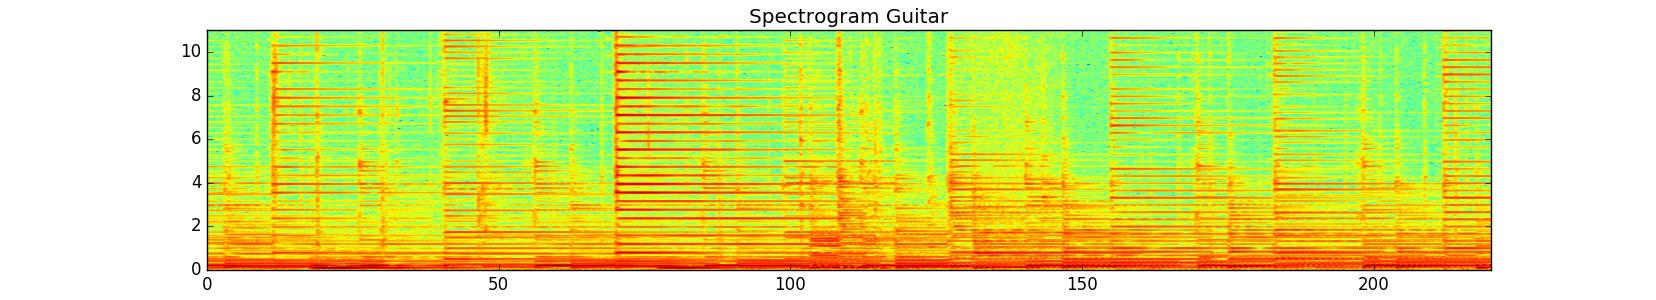
\includegraphics[width=1.25\onecolwid]{figures/guitar}}
    \end{minipage}
    
    \begin{minipage}{1.0\linewidth}
        \centering
        \centerline{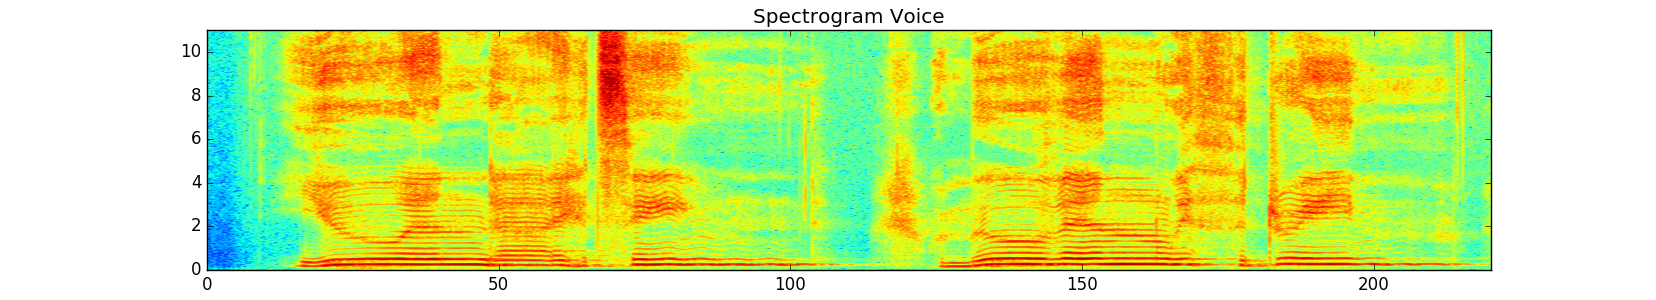
\includegraphics[width=1.25\onecolwid]{figures/singVoice}}
    \end{minipage}
    \begin{minipage}{1.0\linewidth}
        \centering
        \centerline{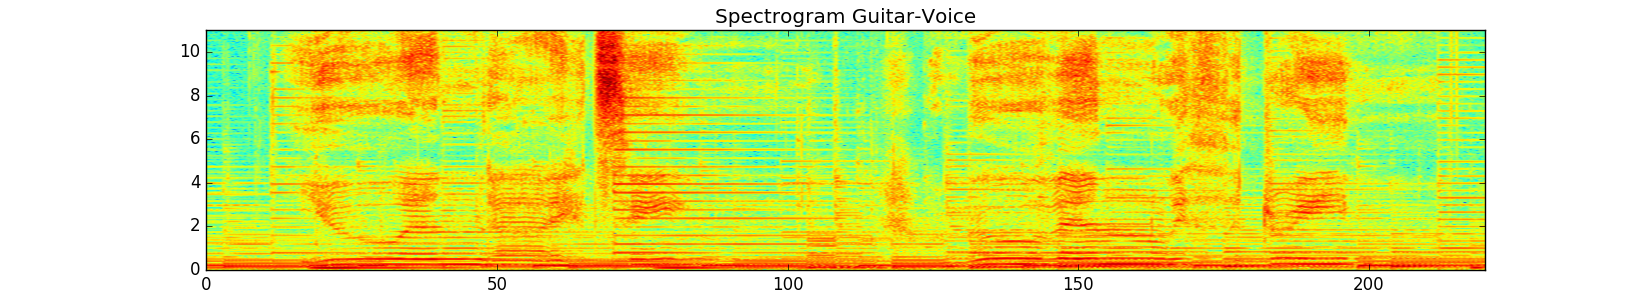
\includegraphics[width=1.25\onecolwid]{figures/gitarVoice}}
    \end{minipage}
    
   
     
    \caption[Spectrograms of guitar and singing voice]{Comparative of the spectrograms of a guitar, a singing voice and its combination. \cite{DS:Weembly}}
    \label{fig:guitarVoice}
\end{figure}

\setbeamercolor{structure}{fg=jblue}
%----------------------------------------------------------------------------------------

\end{column} % End of the first column

\begin{column}{\sepwid}\end{column} % Empty spacer column

\begin{column}{\twocolwid} % Begin a column which is two columns wide (column 2)

\begin{columns}[t,totalwidth=\twocolwid] % Split up the two columns wide column

\begin{column}{\onecolwid}\vspace{-.6in} % The first column within column 2 (column 2.1)

%----------------------------------------------------------------------------------------
%	ACOMUS1
%----------------------------------------------------------------------------------------
\setbeamercolor{block alerted title}{fg=black,bg=YellowOrange} % Change the alert block title colors
\setbeamercolor{block alerted body}{fg=black,bg=white} % Change the alert block body colors
\begin{alertblock}{ACOMUS1}

Acoustic Cover Music Corpus version 1 was constructed based on acoustic covers from amateur artist extracted from YouTube.
The properties of the data are:

\begin{itemize}
\item One accompaniment instrument. 
\item 200 songs with guitar.
\item 40 songs with piano.
\item Only male and female voices, no children.
\item Covers from popular music with no restriction of the style.
\item Songs and artist can have repeated samples.
\item In the English language.
\end{itemize}


\end{alertblock}


%----------------------------------------------------------------------------------------

\end{column} % End of column 2.1


%----------------------------------------------------------------------------------------
%	CORPUS DISTRIBUTION
%---------------------------------------------------------------------------------------- 

\begin{column}{\onecolwid}\vspace{-.6in} % The second column within column 2 (column 2.2)
\setbeamercolor{block alerted title}{fg=black,bg=YellowOrange} % Change the alert block title colors
\setbeamercolor{block alerted body}{fg=black,bg=white} % Change the alert block body colors
\begin{alertblock}{Corpus Distribution}
The characteristics of the data are:
\setbeamercolor{structure}{fg=RedOrange}
    \begin{table}[!htb]
    \caption{Gender distribution of ACOMUS1 corpus}
    \centering
    \label{table:genderACOMUS1}
    \begin{tabular}{l|c c c c}
        \hline
        \multirow{2}{*}{\textbf{Gender}} & 
        \textbf{Unique} & 
        \textbf{Total} & 
            \multicolumn{2}{c}{\textbf{Instruments}} \\
        {} & \textbf{Singers} & {\textbf{Songs}} & {\textbf{Guitar}} & {\textbf{Piano}}\\
        \hline 
        Female 	& 86 & 115 & 91 & 24 \\
        Male 	& 89 & 125 & 109 & 16
    \end{tabular}
\end{table}
    \input{tables/size_distributions.tex}
\setbeamercolor{structure}{fg=jblue}    

\end{alertblock}


\end{column} % End of column 2.2

\end{columns} % End of the split of column 2 - any content after this will now take up 2 columns width

\centering Currently, only 50\% of the ACOMUS1 database is annotated and segmented.


%----------------------------------------------------------------------------------------
%	SEPARATED LINE
%----------------------------------------------------------------------------------------
 \begin{flushleft}
     \vskip-1cm
     \begin{tikzpicture}[remember picture,overlay]
     \shade [inner color=black,outer color=black]
     (0,0) rectangle (\textwidth,0.3cm);
     \end{tikzpicture}
    \end{flushleft}

\begin{columns}[t,totalwidth=\twocolwid] % Split up the two columns wide column
   
%----------------------------------------------------------------------------------------
%	BASEBAND DATA
%----------------------------------------------------------------------------------------   
    
\begin{column}{\onecolwid}\vspace{-.6in} % The first column within column 2 (column 2.1)
\begin{block}{Baseline}
    These are the characteristics of the ACOMUS1 database distribution when generating baseline results: 
\begin{itemize}
    \item Data was separated into groups of 20 songs each. 
    \item Versions of the same song were grouped together.
    \item All song of same artist were grouped together.
    \item WER 92.70\% in bigram and triphone model with SAT speaker adaptation.
\end{itemize}

\end{block}
\end{column}
%----------------------------------------------------------------------------------------
%	AUGMENTATED DATA
%----------------------------------------------------------------------------------------
\begin{column}{\onecolwid}\vspace{-.6in}
\begin{block}{Training Data Augmentation}
    Several experiments were performed with different augmented training  data:
    \begin{enumerate}
        \item Pitch modifications.
        \item Tempo modifications.
        \item Pitch plus Tempo without combinations.
        \item Pitch plus Tempo with combination
    \end{enumerate}
\end{block}

\end{column}
\end{columns}
%----------------------------------------------------------------------------------------



%----------------------------------------------------------------------------------------
%	IMPORTANT RESULT
%----------------------------------------------------------------------------------------

%\begin{alertblock}{Important Result}

%\end{alertblock} 

%----------------------------------------------------------------------------------------

%----------------------------------------------------------------------------------------
%	KALDI 
%---------------------------------------------------------------------------------------- 
%\begin{columns} % Split up the two columns wide column
  
%    \begin{column}{\onecolwid}\vspace{-.6in} % The first column within column 2 (column 2.1)
\begin{block}{Kaldi ASR system}
    \centering
     \input{diagrams/diag_Kaldi.tex}
     
 \end{block}       
       
    
        
        
    %\end{column} % End of the second column

%\end{columns}

\end{column} % End of the second column

\begin{column}{\sepwid}\end{column} % Empty spacer column

\begin{column}{\onecolwid} % The third column


%----------------------------------------------------------------------------------------
%	RESULTS     
%----------------------------------------------------------------------------------------


\begin{block}{Results}
Pitch modification was the only augmentation method that showed a slight increase in performance receiving a 88.33\% WER training DNN sMBR model.
This results can be explained by:
    \begin{itemize}
        \item Mixed reverberation of voice and guitar when using different microphones. 
        \item Harmonic coupling with the background instrument(s) (Fig. \ref{fig:guitarVoice}).
    \end{itemize}
    
 \input{tables/augmentedDataResults.tex}   
%  \input{tables/results.tex}   
    

    
\end{block}

%----------------------------------------------------------------------------------------
%	CONCLUSION           
%----------------------------------------------------------------------------------------

\begin{block}{Conclusion}

ACOMUS1 showed to be a proper corpus for use in ASR on acoustic cover music with guitar and piano instrumentation.
Nevertheless, the first experiments on lyric transcriptions resulted in a high 88\% WER which could be attributed to the coupling reverb of the instrument and voic.
Additional analysis in the pitch augmentation may lead to a better performance.

\end{block}

%----------------------------------------------------------------------------------------
%	ADDITIONAL INFORMATION
%----------------------------------------------------------------------------------------

%\begin{block}{ACOMUS1 projections}

%Increase the size of ACOMUS1 corpus with mayor examples of reverb, loudness, background instruments and singing styles can expand the different uses for this kind of corpus.
%\begin{itemize}
%\item Increase annotations to 1000 guitar and 500 piano songs.
%\item Extend the background instrumental with violin.
%\end{itemize}

%\end{block}

%----------------------------------------------------------------------------------------
%	REFERENCES
%----------------------------------------------------------------------------------------

\begin{block}{References}

\nocite{*} % Insert publications even if they are not cited in the poster
\small{\bibliographystyle{unsrt}
\bibliography{bib/DS_Weembly} 
\vspace{0.75in}}

\end{block}

%----------------------------------------------------------------------------------------
%	ACKNOWLEDGEMENTS
%----------------------------------------------------------------------------------------

%\setbeamercolor{block title}{fg=red,bg=white} % Change the block title color

%\begin{block}{Acknowledgements}

%\small{\rmfamily{My supervisor, Dr. Jon Barker for his guidance during my research project}} \\

%\end{block}


%----------------------------------------------------------------------------------------
%	CONTACT INFORMATION
%----------------------------------------------------------------------------------------

%\setbeamercolor{block alerted title}{fg=black,bg=gray!60} % Change the alert block title colors
%\setbeamercolor{block alerted body}{fg=black,bg=white} % Change the alert block body colors

%\begin{alertblock}{Contact Information}

%\begin{itemize}
%\item Web: \href{http://www.university.edu/smithlab}{http://www.university.edu/smithlab}
%\item Email: \href{mailto:gerardo.roa@gmail.com}{gerardo.roa@gmail.com}
%\end{itemize}

%\end{alertblock}



%----------------------------------------------------------------------------------------

\end{column} % End of the third column

\end{columns} % End of all the columns in the poster

\end{frame} % End of the enclosing frame

\end{document}
